
\documentclass{article}
\usepackage{glossaries}
\usepackage{cite}
\usepackage{color}
\usepackage[english]{babel}
\usepackage{filecontents}
\usepackage[dvipsnames]{xcolor}
\usepackage[numbers,sort&compress]{natbib}
\usepackage{ifthen}
\usepackage{pdfpages}
\usepackage{listings}

\makeglossaries

\newglossaryentry{migration}{
    name={migration},
    description={Migration is the ability to switch to a new version, platform, or physical location \cite{what-is-migration}. This term come from database management, but is also used in other computer science fields.
    }
}

\newglossaryentry{dns}{
    name={DNS},
    description={Domain Name System, used to resolve internet addresses into human readable domain names}}

\newglossaryentry{partition}{
    name={partition},
    description={Bill Calkins defines partition as "Disks are divided into regions called “disk slices” or “disk partitions.” A slice is composed of a single range of contiguous blocks. It is a physical subset of the disk (except for slice 2, which represents the entire disk)."\cite{what_is_partition} }
}

\newglossaryentry{virtual_machine}{
    name={virtual machine},
    description={Oracle Corporation defines it "as a virtualized operating system with its associated software and applications"\cite{what_is_virtual_machine}
    }
}

\newglossaryentry{IT}{
    name={I.T.},
    description={or Internet Technology is defined by Techopedia as use of computers, storage networking and other devices and a variety of other hardware with the purpose of exchanging digital information \cite{techopedia-it-definition}
    }
}

\newglossaryentry{standup}
{
    name=stand-up,
    description={A daily team meeting where every team member gives an overview of done tasks, current tasks and any future work that needs to be done by that member. }
}

\newglossaryentry{bash}
{
    name=bash,
    description={Bourne Again SHell, a UNIX command line virtual shell language}
}

\newglossaryentry{open-source}
{
    name={open-source},
    description={Software that makes its code openly available, allows derived work without restrictions and its distribution is done freely}
}

\newglossaryentry{operating-system}
{
    name={operating system},
    description={The platform on which all user and system software is running. Examples are Windows, Linux, OSX, Android, iOSX}
}

\newglossaryentry{ssh}{
    name={ssh},
    description={
        SSH: secure shell, a network protocol that allows a remote connection to a terminal
    }
}

\newglossaryentry{natnetwork}{
    name={NAT network},
    description={
        A technique where one IP address is mapped to more internal ip addresses, used for security and reduced number of ips. \cite{whatisnat}
    }
}

\newglossaryentry{ipaddress}{
    name={IP address},
    description={
        An identifier that helps locating a resource on the network, usually represents a computer device connected to a network
    }
}

\newglossaryentry{api}{
    name={API},
    description = {
        Application Programmable interface, usually a way for exposing features of a certain program to the developer. Often used to automate a task.
    }
}

\newglossaryentry{vagrant}{
    name={Vagrant},
    description = {
        Vagrant provides easy to configure, reproducible, and portable work environments built on top of industry-standard technology and controlled by a single consistent workflow to help maximize the productivity and flexibility of you and your team. \cite{vagrant-definition}
    }
}

\newglossaryentry{puppet}{
    name={puppet},
    description={
        Open source Puppet helps you describe machine configurations in a declarative language, bring machines to a desired state, and keep them there through automation.\cite{puppet-definition}
    }
}

\newglossaryentry{ruby-on-rails}{
    name={Ruby On Rails},
    description={
        Rails is a web application development framework written in the Ruby language. It is designed to make programming web applications easier by making assumptions about what every developer needs to get started. It allows you to write less code while accomplishing more than many other languages and frameworks.\cite{ruby-on-rails-definition}
    }
}

\newglossaryentry{ruby}{
    name={ruby},
    description={
        A dynamic, open source programming language with a focus on simplicity and productivity. It has an elegant syntax that is natural to read and easy to write.\cite{ruby-definition}
    }
}

\newglossaryentry{html}{
    name={html},
    description={
        Hypertext Markup Language, used for displaying web page
    }
}

\newglossaryentry{ram}{
    name={RAM},
    description={Random Access Memory, also main memory, is a computer hardware component that stores information for fast retrieval.}
}

\newglossaryentry{cpu}{
    name={CPU},
    description={Central Processing Unit, the hardware component that is responsible for executing instructions, evaluate expressions and perform algebraic operations.}
}

\newglossaryentry{gpu}{
    name={GPU},
    description={Graphical Processing Unit, a computer hardware component that specialises in processing highly parallel instructions.}
}

\newglossaryentry{kernel}{
    name={kernel},
    description={Is the core component of an operating system that provides all the services necessary for every component of the system.}
}

\newglossaryentry{vsphere}{
    name={vSphere},
    description={ Is a technology used to manage large collections of infrastructure (such as CPUs, storage, and networking) as a seamless and dynamic operating environment, and also manages the complexity of a datacenter\cite{vsphere-definition}
    }
}

\newglossaryentry{xeon}{
    name={Xeon},
    description={ The Xeon processor family is Intel's server grade processors
    }
}

\newglossaryentry{vmware}{
    name={VmWare},
    description={VMware is the leader in so-called virtual machine software, it is also the name of the product that the company produces \cite{vmware-definition}
    }
}

\newglossaryentry{virtualbox}
{name={virtualbox},
    description={Open-source virtualisation technology created by Oracle}
}

\newglossaryentry{amazon-web-services}{
    name={Amazon Web Services},
    description={Amazon's cloud infrastructure as a service
    }
}

\newglossaryentry{azure}{
    name={Azure},
    description={Microsoft's cloud infrastructure as a service
    }
}








\newglossaryentry{gem}{
    name={gem},
    description={Ruby programming language term for module or package
    }
}

\newglossaryentry{distribution}{name={distribution},
    description={Is a term that describes a Linux operating system with associated packages and pre-installed software
    }
}

\newglossaryentry{netmask}{name={network mask},
    description={A netmask is a 32 bits field whose p high order bits are set to 1 and the low order bits are set to 0. The number of high order bits set 1 indicates the length of the subnet identifier. Netmasks are usually represented in the same dotted decimal format as IPv4 addresses. \cite[p.143]{netmask-definition}
    }
}


\let\oldcite=\cite
\renewcommand\cite[1]{\ifthenelse{\equal{#1}{_NEEDED_}}{[citation~needed]}{\oldcite{#1}}}
\renewcommand*{\glstextformat}[1]{\textcolor{blue}{#1}}
% ENDCUSTOMMACROS

\definecolor{Mycolor2}{HTML}{4a4a4a}

\begin{document}
\section{Work}

A hypervisor is a computer software or hardware that creates the platform layer to a virtual machine and makes it possible to host multiple instances with different configurations \cite{ibmvirtualisation}.

Initially, the plan was to use a hypervisor virtualisation solution such as \gls{virtualbox} and \gls{vmware} just by themselves, and use the \gls{bash} shell scripting language to interface directly with them. A decision was made to use Virtualbox, as it is an \gls{open-source} software solution, has strong community, allows third party plug-ins and is a solution build by Oracle - a large software corporation. There are other alternatives (gnome boxes, CHROOT), but what influenced the choice is that virtualbox is configurable and can be controlled from the command-line straight out of the box. Another deciding factor was also the extensibility that it offers with third party modules developed by the community and the core team (guest additions, virtualbox standard development kit).

Another reason for not choosing a more unpopular technology is due to the willingness of an adopter to switch their entire virtual infrastructure to it. The Virtualbox software is very popular \cite{_NEEDED_}, and as such, it would make the transition to the platform easier.

During the period when researching Virtualbox, the command-line \gls{api} documentation was used extensively. In the process, a variety of customisable parameters when building a virtual machine were discovered, like the different possibilities in setting up networks (private, network shared, host only, etc.), exposing ports, as well as different hardware configurations (RAM, hard drive, CPU count). After using the command line tools and writing a simple shell scripts for managing creation of different resources, a decision was made to use a tool that manages the different technical details of each virtual machine. Instead of building the manager from scratch, an open-source hypervisor provisioner software was used instead. The tools is called \gls{vagrant}.

\subsection{Vagrant}
Vagrant by Hashicorp, is a tool built by a company specialising in easy virtual machine configuration management and set-up Their \gls{api} provides the following features.

\begin{itemize}
	\item
	Allow the administrator to create a \gls{vagrant} configuration file (called Vagrantfile), which describes end-to-end each operation that will be performed to the virtual machine instance (including the Linux distribution that will get installed on it).
	\item
	Create a system compatible with their platform starting from a bare configuration and incrementally building a bespoke instance. These instances can be managed and shared on the internet.
	\item
	Managing network interfaces
	\item
	Configure ports
	\item
	Allow port access to adapter network (in private networks)
	\item
	Create a custom machine compatable with the platform
	\item 
	Kick-start automation by running one of the supported automation frameworks (chef, puppet)
\end{itemize}

\subsection{Workflow}
The framework that was created uses a \gls{virtual_machine} instance object and authenticated user that owns it. When the user fills the web form with the relevant information, it will pass the configuration values directly to a virtual machine class. This class contains a dynamic configuration, which ensures that the solution is distribution agnostic. Here, the term distribution references to the different versions of Linux (Ubuntu, fedora, Centos, arch Linux). Separating dependency specific configuration by sub-classing a configuration object allows for a quick way for the project to be extended to accommodate for new distributions.

To do so, folder with the name of the new distribution must be placed in lib/configurations that describes the configuration specific settings that include updating and installing common software packages.

The framework also uses UNIX environmental variable to manage infrastructure state. For the  purpose of developing and testing, I have created two main isolated environments - testing and development.
The most notable usage of such environment is the virtual host-only network that ensures that the virtual interfaces do not clash during testing and development. The two interfaces are \texttt{vboxnet0} and \texttt{vboxnet1}. One is for general purpose development, the another is for testing. A special host-only adapter is used to have an isolated ip range that is network agnostic, for example, on a \gls{natnetwork}, some IP addresses might be reserved or used, this case will cause a clash and the virtual machine will not be reachable.

\subsection{Architecture}
When considering the architecture of the system, a list of factors were evaluated when building the solution. One is having few well consolidated moving parts, ensuring flexibility and extensibility. For that purpose the programming language \gls{ruby} was chosen. It is a suitable for system automation as it is very expressive and is for the most part platform independent (interpreted). Its suitability comes also from the available tools \gls{vagrant} and \gls{puppet} which allow end-to end integration when developing and testing. The \gls{ruby} programming language also draws inspiration from the Perl programming language. One of the Perl's strengths is its ability to be a more powerful shell scripting language as well as a general purpose language. This is the case as it has quick syntax for executing shell scripts directly and get STDOUT, STDERR and exit-codes quickly. It does also has native implementation of common UNIX tools, like grep, wget and awk (core GNU utilities).\cite{perl-programming-language-shell-scripting}

\begin{figure}
	\vspace{1cm}
	\centering          
	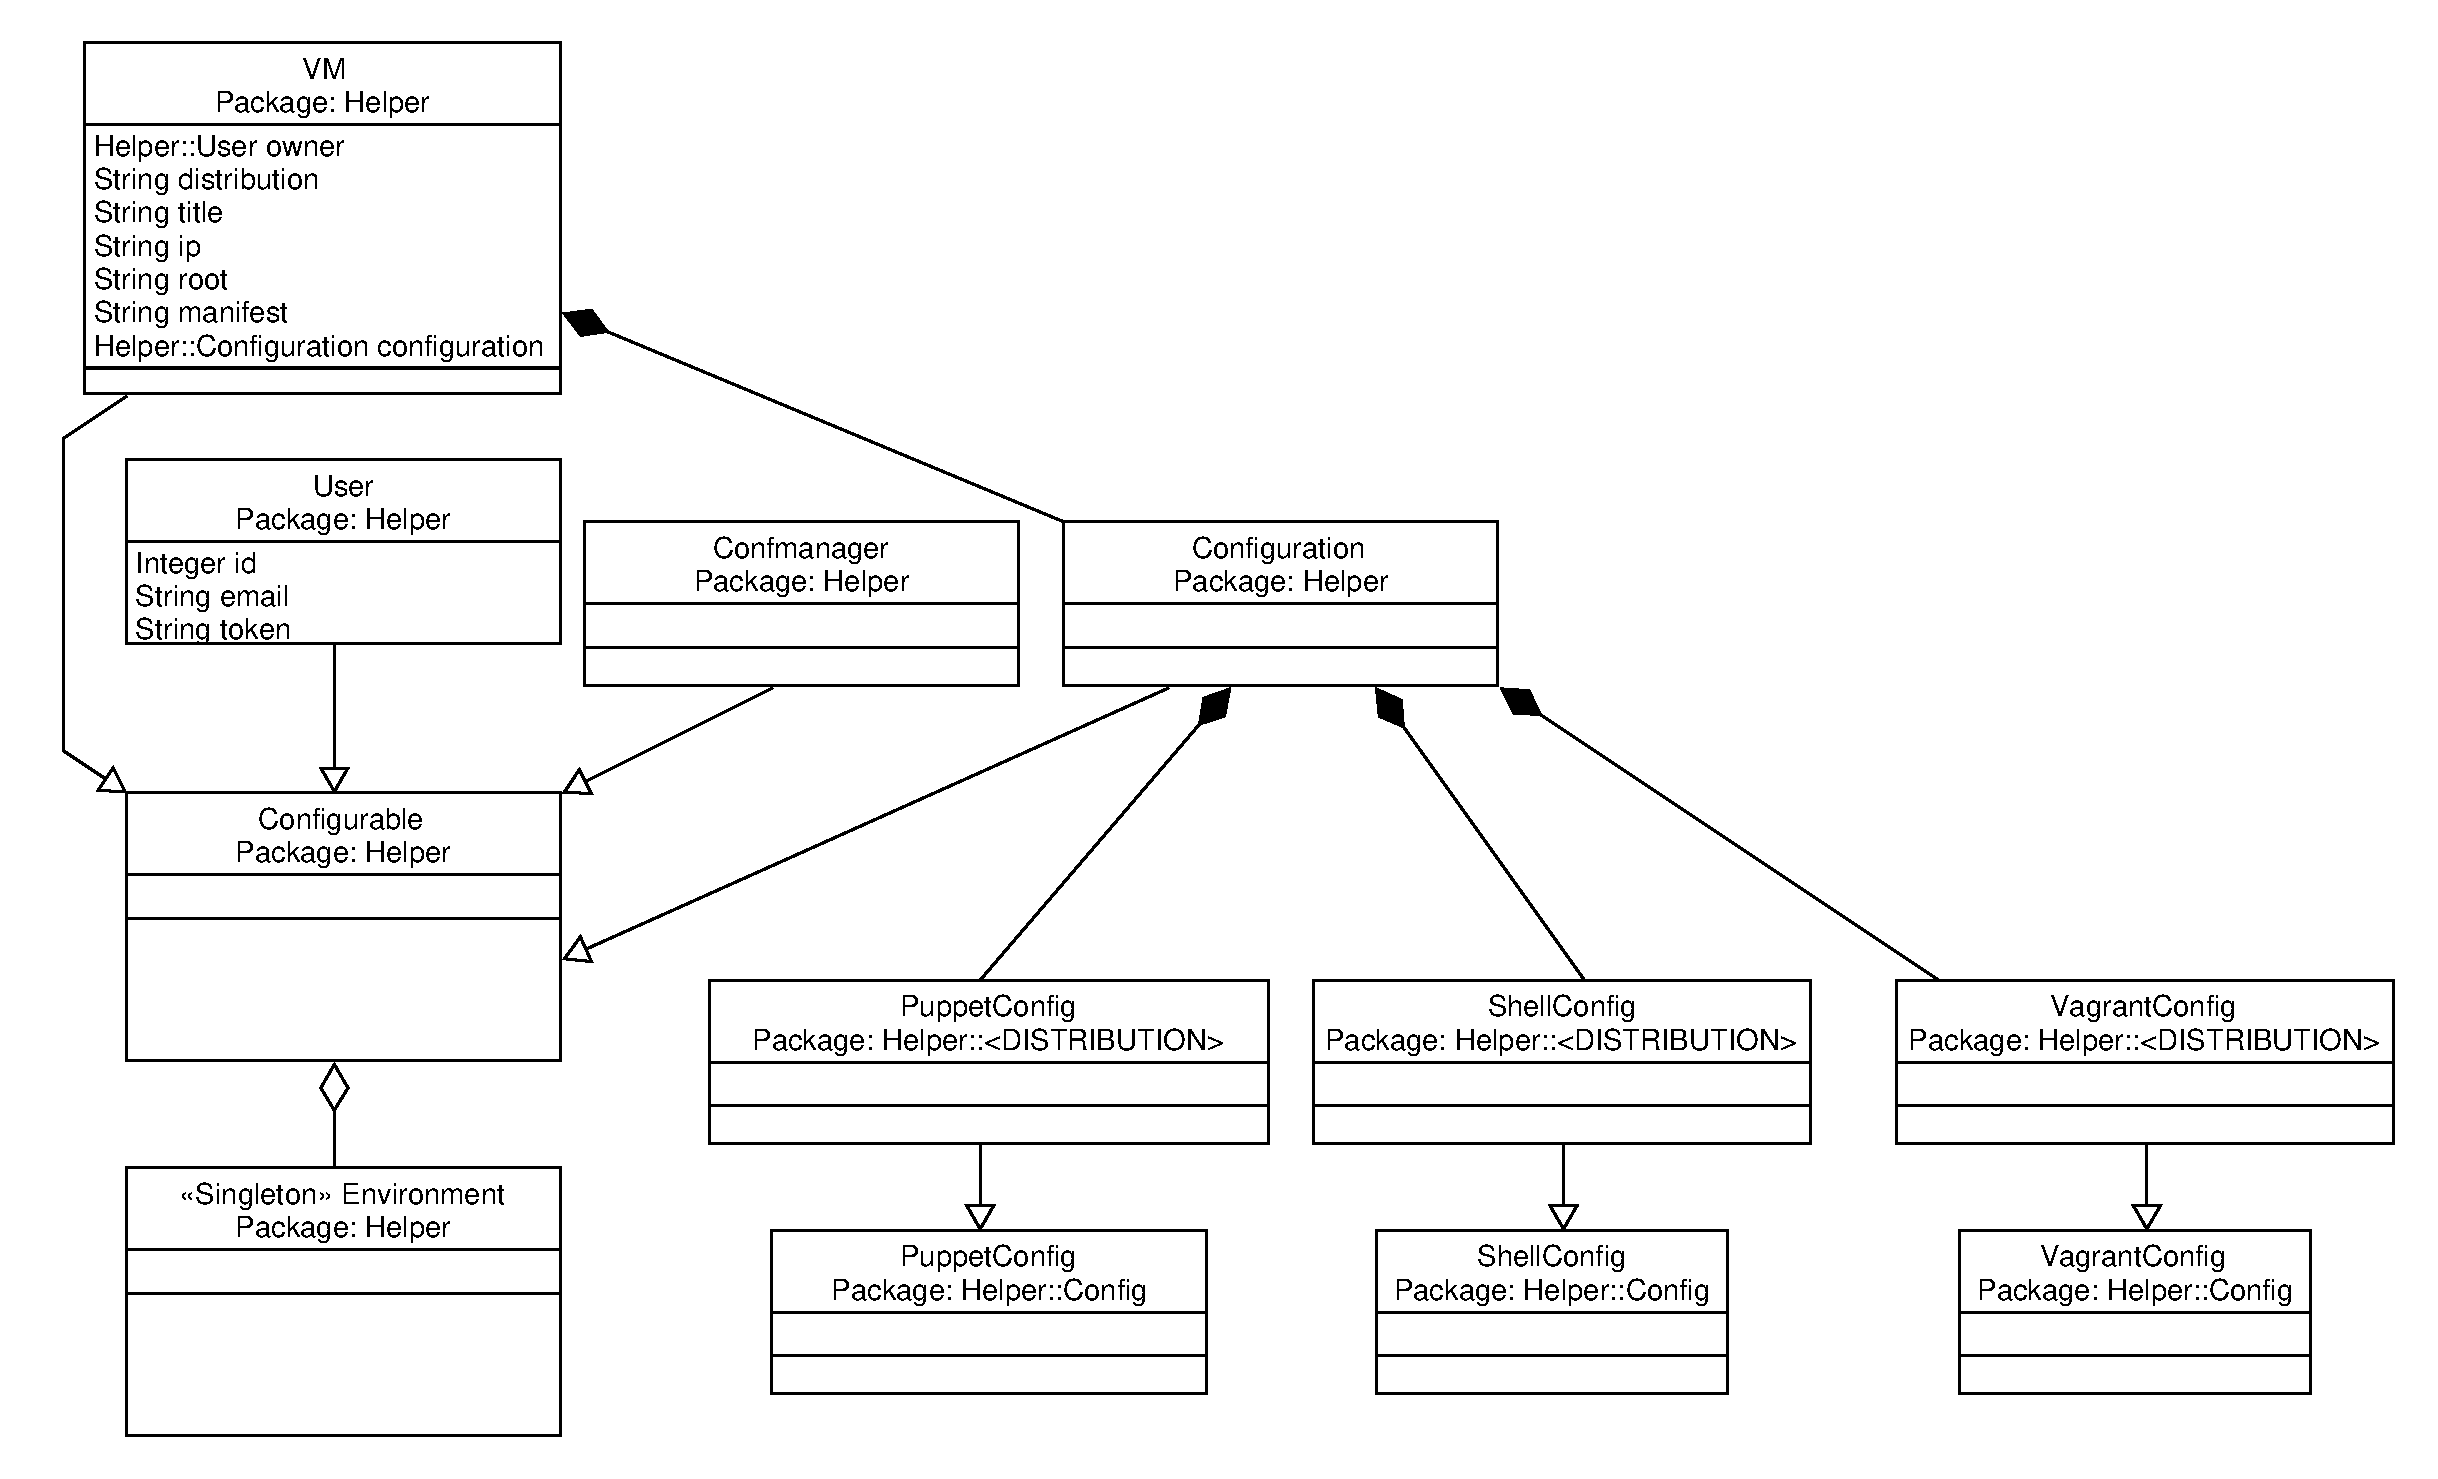
\includepdf[width=1\textwidth]{architecture.pdf}      
	\caption{Diagram of the architecture of deeploy module}
	\label{fig:Test}
	\vspace{3cm}
\end{figure}

%\newpage
%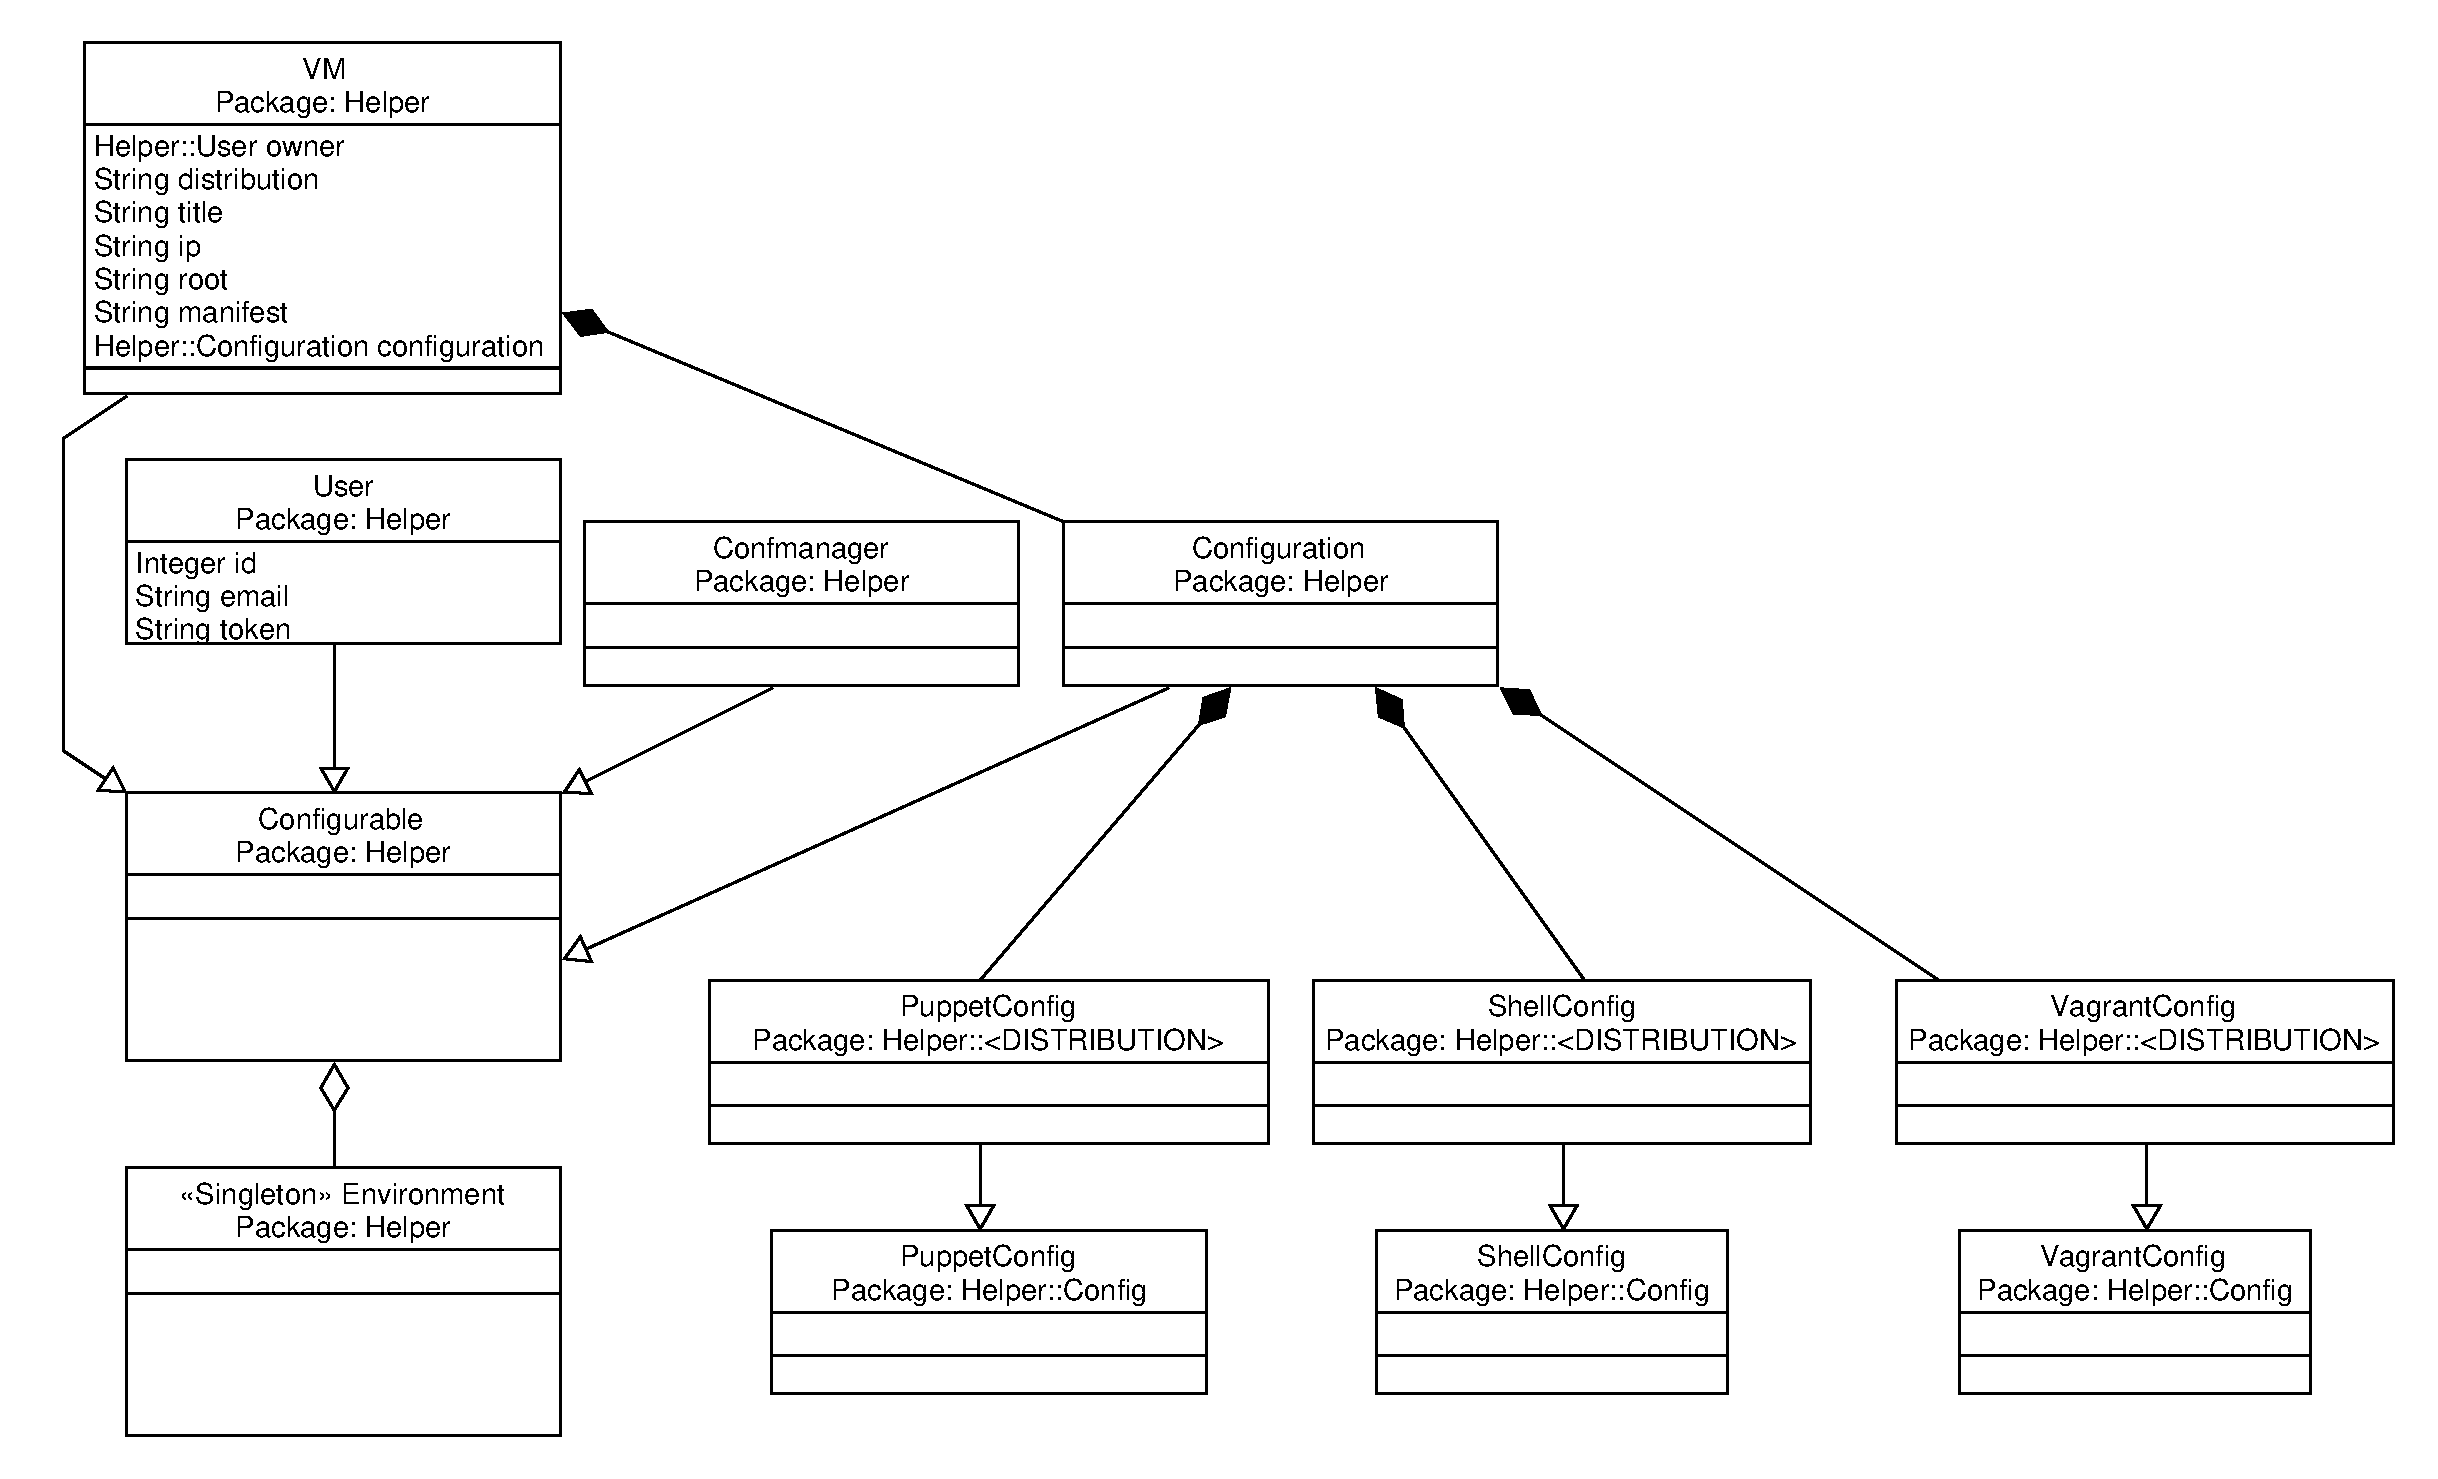
\includepdf{architecture.pdf}

Because the Ruby language draws inspiration and shares similar features with Perl, it makes it a great modern and powerful language to use in this domain-specific problem. The language benefits from it bein written in 1995, and being very mature. For that reason, there is a great amount of online help and third party library of great quality.

\subsection{The deeploy module}

The first component of the work is a ruby module designed specially to act as a back-end for the entire solution. A module is a collection of programming functions and libraries that are bundled together to achieve a particular task. In \gls{ruby}, modules are called gems. For writing my first \gls{gem}, the official ruby guide was used as guide \cite{ruby-official-guide}. 

The file \texttt{lib/deeploy.rb} is what sets up the database connection and bootstraps the whole module by auto-loading every component. To ease integration, the file loads configuration properties from the file \texttt{lib/config/application.yml}. \texttt{Application.yml} contains configuration for production, development and testing, this is to allow separation and configuration of different parameters. The file specifies location of the database file when in development, or it has the database drivers in production with information about connection parameters. The file also describes the network interfaces to be used in each environment.

\texttt{lib/deeploy.rb} has a helper method that returns the current network interface and \gls{netmask}, this function is responsible for generating \glspl{ipaddress} and also for verifying that the virtual network is up and running. It does so by issuing commands for bringing up the virtual networks \texttt{vboxnet} up, then using network sockets to extract relevant information. This function is the programatic equivalent to the command \texttt{ifconfig or ipconfig}.

The file also contains a static function that returns a map of all supported distributions and the associated \gls{vagrant} machine. The function is helpful when validating creation, and will error out if the \gls{distribution} name is not in the list. When extending the supported distribution, this function needs updating. 

Similarly to the supported \glspl{distribution} function, there is a static function to return the supported packages list, used for displaying the options and validating unsupported packages.

The module provides a function slugify, its purpose is to convert string with special characters and spaces to a set of words and dashes, non-ASCII characters are stripped.

\gls{ipaddress} helper function checks if the supplied  is part of the current network by using ruby's \texttt{ipaddr} build in module. 

The file \texttt{lib/vm.rb} contains the code for managing the virtual machine instances, the class is called \texttt{Deeploy::Configurable::VM}. The class inherits from \texttt{Configurable}. Calling \texttt{VM.new} contains validators that raise errors upon initialising the class inappropriately. 
The method is responsible for specifying the distribution, available resources, configuration destination, name of the instance, packages, open ports and prepares it for creation. A design decision was made to allow a machine to be configured with the \texttt{new} operator and then created by issuing \texttt{machine\_instance.build()}.

The method \texttt{VM.alive()} verifies if the machine is alive by trying to listen on \gls{ssh} port, if it fails within a time-out, the machine is updated to state of not alive.	

\texttt{VM.get()} is used when performing power up, power down and destroy virtual machines. It queries the database and discovers everything about the instance, from packages, to \gls{ram} and location of configuration files.

The virtual machine is built only when an instance is initialised properly by calling \texttt{VM.new} with the correct arguments and then invoke \texttt{VM.build()}. The design decision to have a separate functionality of bootstrapping instances was mainly for cleaner testing by compartmentalising the components into smaller elements. The \texttt{build} method also accepts a boolean argument. This argument tells the current build if it is in "dry-run" mode. The mode, the machine will create directories and configuration without actually bringing the instance up and running. This is again, done for testing reasons - they verify that different \glspl{distribution} have appropriate configurations.

During the invocation of the \texttt{build} method, a \gls{bash} shell is forked and it executes the \gls{vagrant} command that brings it on-line and installs all dependencies. The shell command also tells the script to write all output to a text file in the machine directory, the file is called \texttt{vagrant.log}. Because the process takes a long time to finish, an axillary function \texttt{_wait_on_build} is used. This function constantly goes through the contents of the log file and checks what is the current building state of the instance. Typical states are building the base, installing puppet, setting up dependencies, installing packages and the state everything has finished.


TALK ABOUT CHDIR ISSUE THREAD SAFE AND ABOUT HEALTH MONITORING DEAMON INSTEAD OF CHECKING EVERYTIME DUE TO THE SLOWDOWN

\bibliography{work}
\renewcommand{\bibname}{}

\end{document}

\begin{filecontents*}{work.bib}
    @online{ruby-official-guide,
        author = {RubyGem Team},
        title = {Make your own gem},
        url = {http://guides.rubygems.org/make-your-own-gem/},
        urldate = {2011},
        note = {Accessed: April 13, 2017}
    }

    @online{netmask-definition,
        author = {Olivier Bonaventure},
        title = {Computer Networking : Principles, Protocols and Practice},
        url = {https://www.saylor.org/site/wp-content/uploads/2012/02/Computer-Networking-Principles-Bonaventure-1-30-31-OTC1.pdf},
        urldate = {2011},
        note = {Accessed: April 13, 2017}
    }
    
\end{filecontents*}
